\documentclass[uplatex,12pt]{jsarticle}
\usepackage[dvipdfmx]{graphicx}
\usepackage{url}
\usepackage{listings,jlisting}
\usepackage{ascmac}
\usepackage{amsmath,amssymb}

%ここからソースコードの表示に関する設定
\lstset{
  basicstyle={\ttfamily},
  identifierstyle={\small},
  commentstyle={\smallitshape},
  keywordstyle={\small\bfseries},
  ndkeywordstyle={\small},
  stringstyle={\small\ttfamily},
  frame={tb},
  breaklines=true,
  columns=[l]{fullflexible},
  numbers=left,
  xrightmargin=0zw,
  xleftmargin=3zw,
  numberstyle={\scriptsize},
  stepnumber=1,
  numbersep=1zw,
  lineskip=-0.5ex
}
%ここまでソースコードの表示に関する設定

\title{知能プログラミング演習II 課題5}
\author{グループ8\\
  29114116 増田大輝\\
}
\date{2019年12月2日}

\begin{document}
\maketitle

\paragraph{提出物} rep5, group08
\paragraph{グループ} グループ8

\paragraph{メンバー}
\begin{tabular}{|c|c|c|}
  \hline
  学生番号&氏名&貢献度比率\\
  \hline\hline
  29114003&青山周平&NoData\\
  \hline
  29114060&後藤拓也&NoData\\
  \hline
  29114116&増田大輝&NoData\\
  \hline
  29114142&湯浅範子&NoData\\
  \hline
  29119016&小中祐希&NoData\\
  \hline
\end{tabular}



\section{課題の説明}
\begin{description}
\item[必須課題5-1] 目標集合を変えてみたときに,動作が正しくない場合があったかどうか,実行例を示して考察せよ.
また,もしあったならその箇所を修正し,どのように修正したか記せ.
\item[必須課題5-2] 教科書のプログラムでは,オペレータ間の競合解消戦略としてランダムなオペレータ選択を採用している.
これを,効果的な競合解消戦略に改良すべく考察し,実装せよ.
改良の結果,性能がどの程度向上したかを定量的に(つまり数字で)示すこと.
\item[必須課題5-3] 上記のプランニングのプログラムでは,ブロックの属性(たとえば色や形など)を考えていないので,色や形などの属性を扱えるようにせよ.ルールとして表現すること.
例えば色と形の両方を扱えるようにする場合,Aが青い三角形,Bが黄色の四角形,Cが緑の台形であったとする.
その時,色と形を使ってもゴールを指定できるようにする("green on blue" や"blue on box"のように)
\item[必須課題5-4] 上記5-2, 5-3で改良したプランニングシステムのGUIを実装せよ.
ブロック操作の過程をグラフィカルに可視化し,初期状態や目標状態をGUI上で変更できることが望ましい.
\item[発展課題5-5] ブロックワールド内における物理的制約条件をルールとして表現せよ.
例えば,三角錐(pyramid)の上には他のブロックを乗せられない等,その世界における物理的な制約を実現せよ.
\item[発展課題5-6] ユーザが自然言語(日本語や英語など)の命令文によってブロックを操作したり,初期状態/目標状態を変更したりできるようにせよ.
なお,命令文の動詞や語尾を1つの表現に決め打ちするのではなく,多様な表現を許容できることが望ましい.
\item[発展課題5-7] 3次元空間 (実世界) の物理的な挙動を考慮したブロックワールドにおけるプランニングを実現せよ.
なお,物理エンジン等を利用する場合,Java以外の言語のフレームワークを使って実現しても構わない.
\item[発展課題5-8] 教科書3.3節のプランニング手法を応用できそうなブロック操作以外のタスクをグループで話し合い,新たなプランニング課題を自由に設定せよ.
さらに,もし可能であれば,その自己設定課題を解くプランニングシステムを実装せよ.
\end{description}

\section{必須課題5-3}
\begin{screen}
    上記のプランニングのプログラムでは,ブロックの属性(たとえば色や形など)を考えていないので,色や形などの属性を扱えるようにせよ.ルールとして表現すること.
    例えば色と形の両方を扱えるようにする場合,Aが青い三角形,Bが黄色の四角形,Cが緑の台形であったとする.
    その時,色と形を使ってもゴールを指定できるようにする("green on blue" や"blue on box"のように)
\end{screen}
\subsection{手法}
ブロックの属性を扱えるようにするために,まずはルールによってブロックと属性の関係を表現し,それらの関係を保持する必要がある.
その上で,属性によって表現されたゴールや,初期状態をブロックによる表現に変換し,後ろ向き推論を行う方針とした. \\
ここで,ブロックの属性によってゴールを表現する場合,そのまま後ろ向き推論を行うと,同一ブロックの異なる属性による表現がワーキングスペースに含まれる場合などへの対応が非常に複雑となる.
したがって,入力されたルールと初期状態はあらかじめ属性表現をブロックに変換することで,もとの後ろ向き推論が正常に機能するような実装を行うものとする.

\subsection{実装}
まず,属性を扱うクラスAttributionsを作成した.
Attributionsクラスの変数としてHashMap<String,String>型のattributions,List<String>型のrulesがある.
それぞれ,属性とブロックの関係(属性が主キー)の集合,ルールの集合に対応する.
このAttributionsクラスには以下の3つのコンストラクタが存在し,全て上記変数への操作を行うものであるが,それぞれに次のような用途がある.

\begin{description}
    \item[Attributions()] テスト用のデフォルトコンストラクタ.デフォルトのルールが用意されている.ルールは自然言語で記述.
    \item[Attributions(List \textless String\textgreater rules)] 自然言語で記述されたルールをもとに属性とブロックの関係を構築する.
    \item[Attributions(HashMap \textless String, String\textgreater attributions)] あらかじめ,属性とブロックの関係が構築された状態のものを受け取る.
\end{description}
ただし,自然言語で記述されているものは,"ブロック is 属性"の形で表現されているものを扱うものとする.
例えば,"A is blue"と記述されたものを受理する. \\

次に,自然言語から属性とブロックの関係を構築するメソッドaddAttribution(String attributionState)についての説明を行う.
このメソッドは上記コンストラクタAttributions()とAttributions(List \textless String\textgreater rules)から呼び出される.
これらのコンストラクタからはrulesの各要素を引数として渡すものとする.
addAttributionメソッドは仮引数attributionStateでこれらを受け取り,"ブロック is 属性"を空白で分割したリストの第二要素が"is"である場合に,attributionsに関係を加える.
この時,属性を主キーとし,ブロックを紐づけられるオブジェクトとする. \\
すなわち,"A is blue"とした場合には,第二要素は"is"であるので"blue"を主キーとして,"A"と紐づけられることとなる. \\

以上により,属性を持つブロックを扱うための下準備が整った. \\

続いて,attributionsに格納された属性とブロックの関係をゴールリストや初期状態のリストに適応するためのメソッドeditStatementList(ArrayList<String> statementList)についての説明である.
このメソッドでは,仮引数として渡されたstatementListの各要素について,attributions内に格納されている属性との照合作業が行われ,属性がある場合には紐づけられたブロック名に置き換えられる作業が行われる.
以下にメソッドのソースコードを示す.
\begin{lstlisting}[caption=editStatementListメソッドの実装, label=mid]
    ArrayList<String> editStatementList(ArrayList<String> statementList) {
		System.out.println("++++++ EditStatement ++++++");
		ArrayList<String> newStatementList = new ArrayList();
		for (String statement: statementList) {
			List<String> tokens = Arrays.asList(statement.split(" "));
			String newStatement = "";
			for(int tokenNum = 0; tokenNum < tokens.size(); tokenNum++) {
				String token = tokens.get(tokenNum);
				if(attributions.containsKey(token)) {
					token = attributions.get(token);
				}
				newStatement += token;
				if(tokenNum < tokens.size()-1) {
					newStatement += " ";
				}
			}
			newStatementList.add(newStatement);
			System.out.println(statement+" =====> "+newStatement);
		}
		return newStatementList;
	}
\end{lstlisting}
特に,9~11行目でHashMapの機能を利用して属性からブロック名を導き出す処理を行っている.

以上によって,自然言語で記述されたルール集合から導出された属性とブロックの関係や与えられた属性とブロックの関係を元にして,
ゴールリストや初期状態のリストに含まれる属性表現をブロック名に統一する処理が完成した.

具体的な利用法は,使用したい任意のコンストラクタによってAttributionsクラスを初期化し,以下のような形で,ゴールリストや初期状態のリストに適用すればよい.
\begin{lstlisting}[caption=editStatementListの利用, label=mid]
    goalList = attributions.editStatementList(initAttributeGoalList());
	initialState = attributions.editStatementList(initAttributeInitialState());
\end{lstlisting}


\subsection{実行例}
以下に,CUI上での実行結果を示す.
ただし,コンストラクタはデフォルトコンストラクタを使用するものとする.
\begin{lstlisting}[caption=ゴールと初期状態に属性を指定した場合の実行結果, label=mid]
    ~/Programming2/Work5
    ●java Planner                                                                                                                                                                                                     【 re-fix/attribute-rule 】
    ========== goal:green on ball ==========
    ========== goal:blue on pyramid ==========
    ++++++ EditStatement ++++++
    green on ball =====> B on C
    blue on pyramid =====> A on B
    ---------- initInitialState:clear blue ----------
    ---------- initInitialState:clear green ----------
    ---------- initInitialState:clear red ----------
    ---------- initInitialState:ontable box ----------
    ---------- initInitialState:ontable pyramid ----------
    ---------- initInitialState:ontable ball ----------
    ---------- initInitialState:handEmpty ----------
    ++++++ EditStatement ++++++
    clear blue =====> clear A
    clear green =====> clear B
    clear red =====> clear C
    ontable box =====> ontable A
    ontable pyramid =====> ontable B
    ontable ball =====> ontable C
    handEmpty =====> handEmpty
    *** GOALS ***[B on C, A on B]
    **B on C
    Place B on C
    *** GOALS ***[clear C, holding B]
    **clear C
    [clear A, clear B, clear C, ontable A, ontable B, ontable C, handEmpty]
    *** GOALS ***[holding B]
    **holding B
    pick up B from the table
    *** GOALS ***[ontable B, clear B, handEmpty]
    **ontable B
    [clear A, clear B, clear C, ontable A, ontable B, ontable C, handEmpty]
    *** GOALS ***[clear B, handEmpty]
    **clear B
    [clear A, clear B, clear C, ontable A, ontable B, ontable C, handEmpty]
    *** GOALS ***[handEmpty]
    **handEmpty
    pick up B from the table
    Place B on C
    [clear A, ontable A, ontable C, B on C, clear B, handEmpty]
    *** GOALS ***[A on B]
    **A on B
    Place A on B
    *** GOALS ***[clear B, holding A]
    **clear B
    [clear A, ontable A, ontable C, B on C, clear B, handEmpty]
    *** GOALS ***[holding A]
    **holding A
    pick up A from the table
    *** GOALS ***[ontable A, clear A, handEmpty]
    **ontable A
    [clear A, ontable A, ontable C, B on C, clear B, handEmpty]
    *** GOALS ***[clear A, handEmpty]
    **clear A
    [clear A, ontable A, ontable C, B on C, clear B, handEmpty]
    *** GOALS ***[handEmpty]
    **handEmpty
    pick up A from the table
    Place A on B
    ***** This is a plan! *****
    pick up B from the table
    Place B on C
    pick up A from the table
    Place A on B
\end{lstlisting}
まず,3・4行目で属性によってゴールが表現されていること示している.
その次に,5~7行目でこれらのゴールを属性からブロック名による表現に変換している.
続いて,8~14行目で属性によって式状態が表現されていることを示している.
先ほどと同様に,15~22行目では,これらの表現を属性によるものからブロック名のみの形に変更している.
したがって,以降の実行結果はブロック名のみを用いた場合と同様となる.

\subsection{考察}
属性を扱うに当たって,初めは属性のまま推論を行い,プランニングを実行できるようにしようと考えた.
しかし,同じブロックの属性であっても,異なる属性同士において,字面だけではマッチングが成功しないことに気が付いた.
例えば"A is blue"と"A is box"がルールとして与えられていたとする.
この時,ゴールが"blue on green"で,状態として"box on green"が保持されているものとする.
本来,blueとboxは同じブロックAの属性であるが,字面の上では,異なる定数として認識される. \\
これらを同一のブロックAを指し示すものとして認識するには,属性からブロックそのものへと変換する機能が必要である.
したがって,変換後のゴール"A on B"と状態"A on B"であればマッチングは成功する. \\
ここで,もう一度属性のまま推論を行う意義を考えることとした.
上記の方法では,マッチングにおいて最終的に属性からブロック名への変換処理を行っている.
ところが,初めから同様に属性をブロック名に変換する手法にすることでもマッチングは可能である.
例えば,あらかじめゴールを"blue on green"から"A on B"に変換し,初期状態を全てブロック名による表現にすることで,プランニング中の状態を"A on B"とする.
結果として,即座に"A on B"と"A on B"のマッチングが行われるようにする. \\
加えて,後者の方がゴールリストと初期状態のリストから属性表現をブロック名に変換するのみであるので,処理も非常にシンプルとなる.
後ろ向き推論の特徴と処理の簡潔さから,後者の手法を採用することにした. \\
複数ある実現方法の中から,既存のプログラムとの相性や論理的な汎用性を考えてもっとも良いと思える方法を選択できたと考えている.


\section{発展課題5-5}
\begin{screen}
    ブロックワールド内における物理的制約条件をルールとして表現せよ.
    例えば,三角錐(pyramid)の上には他のブロックを乗せられない等,その世界における物理的な制約を実現せよ.
\end{screen}
\subsection{手法}
ブロックワールド内における物理的制約条件(以下、禁止制約と表現する)をルールとして表現し,プランニングに反映するために,
課題5-3で作成した属性に関する処理を扱うクラスAttributions内に禁止制約のルールを保持させる方法を考案した.
例えば,"box on pyramid"(三角錐の上に正四面体がある)のようなルールが物理法則に反する禁止制約に当たる. \\
これらの禁止制約のルール集合を,課題5-3で結びつけた「属性とブロックの関係」をもとに,属性を用いた表現からブロックによる表現に置き換える. \\
以上により,ゴールリストやオペレーター適用後の状態とブロックによって表現される禁止制約を比較することで,
物理法則に反する状態を削除することができる.
また,ゴールリストに物理法則に反するものが含まれる場合には,ゴール不成立とする. 

以下に,今回実装した禁止制約の例を示す. \\

\begin{figure}[!hbt]
  \centering
  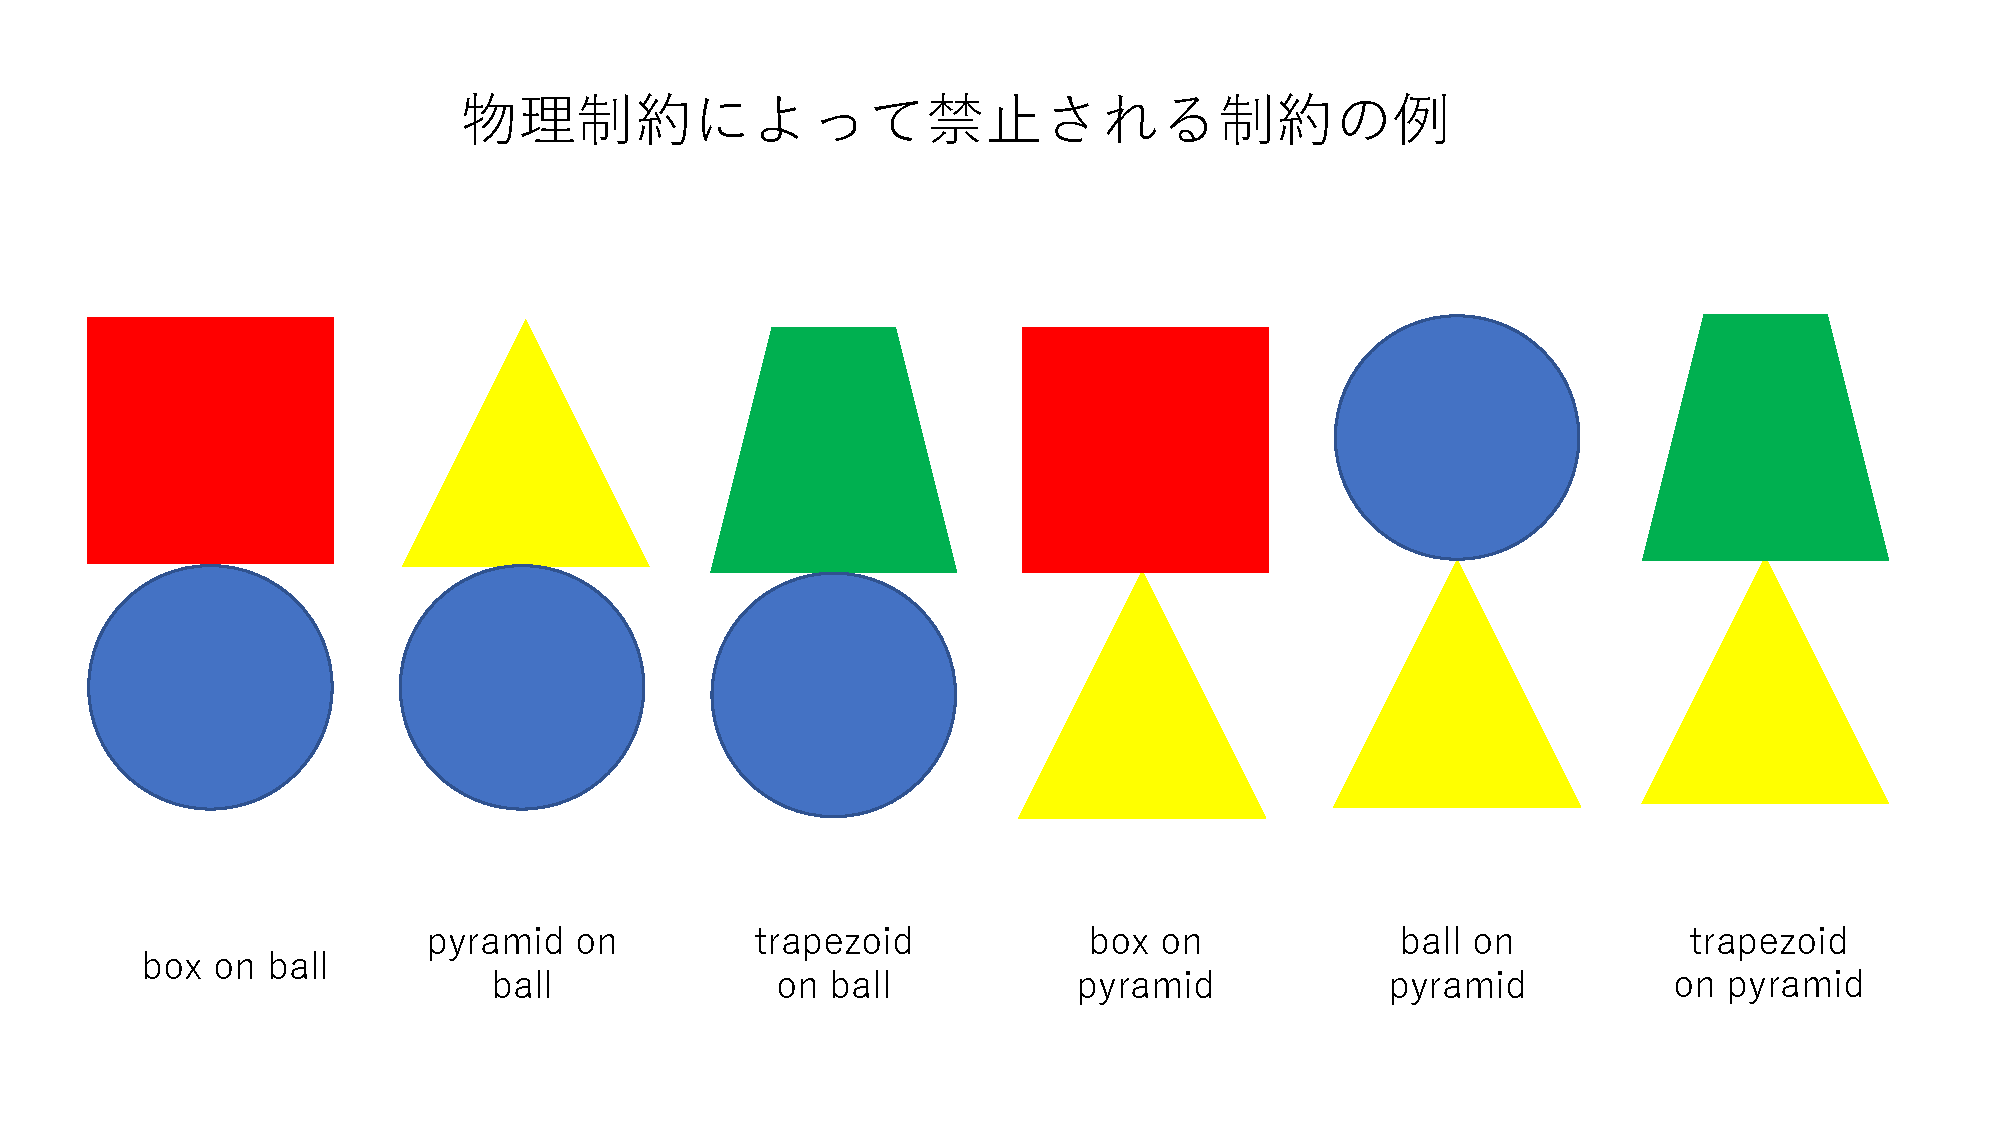
\includegraphics[scale=0.35]{images/prohibit-rules.pdf}
  \caption{物理制約によって禁止される制約の例}
\end{figure}

\subsection{実装}
まず,属性を扱うAttributionsクラス内にArrayList<String>型の禁止制約のルール集合prohibitRulesを保持させる.
このprohibitRulesはコンストラクタから呼び出されるメソッドaddProhibitRules()により禁止制約のルールが追加される. \\
加えて,属性によって表現された禁止制約のルールをブロックによる表現に置き換えたルール集合prohibitBlockStatesも定義する.
prohibitRulesからprohibitBlockStatesに変換を行うに当たっては,課題5-3で作成したメソッドeditStatementListを用いる. \\
次に,状態と禁止制約を比較するメソッドcheckProhibitBlockState(String state)を実装した.
このメソッドを以下に示す.
\begin{lstlisting}[caption=checkProhibitBlockStateメソッドの実装, label=mid]
    private Boolean checkProhibitBlockState(String state) {
		for(String prohibitBlockState: prohibitBlockStates) {
			if(prohibitBlockState.equals(state)) {
				System.out.println("【Warning!:状態"+state+"は禁止制約です!!】");
				return false;
			}
		}
		return true;
	}
\end{lstlisting}
2~7行目に渡って,全ての禁止制約のルール集合の要素と仮引数で受け取った状態を比較する処理を行なっている.
ここで,一つでも禁止制約と一致すると,falseが返却される.
反対に,全ての禁止制約と一致しなかった場合には,trueが返却される. \\
続いて,このcheckProhibitBlockStateメソッドを利用するcheckStates(ArrayList<String> states)メソッドの説明を行う.
このメソッドについても以下に示す.
\begin{lstlisting}[caption=checkStatesメソッドの実装, label=mid]
    ArrayList<String> checkStates(ArrayList<String> states) {
		ArrayList<String> checkedStates = new ArrayList<String>();
		for(String state: states) {
			if(checkProhibitBlockState(state)) {
				checkedStates.add(state);
			}
		}
		return checkedStates;
	}
\end{lstlisting}
3~7行目に渡って,仮引数で受け取った状態集合の各要素をcheckProhibitBlockStateの引数として渡すことで,禁止制約のチェックを行なっている.
結果としてtrueが帰ってきた場合にはチェック済みの状態集合checkedStatesに格納し,falseの場合には格納されない. \\
全ての要素のチェックが終わると,checkedStatesを返却する. \\
checkedStatesメソッドを,変化直後の状態集合に対して使用することによって,物理法則に反する状態を削除することができる.
以上の実装により,禁止制約のブロックワールドへの反映を実現した.

\subsection{実行例}
以下に,CUI上での実行結果を示す.
ただし,コンストラクタはデフォルトコンストラクタを使用するものとする.
\begin{lstlisting}[caption=禁止制約によりゴールが成立しなくなった場合, label=mid]
    ~/Programming2/Work5
    ●java Planner                                                                                                                                                                                                    【 feature/prohibit-rules 】
    ###### Add prohibitRule ######
    ****** ProhibitRule:box on pyramid ******
    ****** ProhibitRule:box on ball ******
    ****** ProhibitRule:ball on pyramid ******
    ****** ProhibitRule:pyramid on ball ******
    ****** ProhibitRule:trapezoid on pyramid ******
    ****** ProhibitRule:trapezoid on ball ******
    ++++++ EditStatement ++++++
    box on pyramid =====> A on B
    box on ball =====> A on C
    ball on pyramid =====> C on B
    pyramid on ball =====> B on C
    trapezoid on pyramid =====> trapezoid on B
    trapezoid on ball =====> trapezoid on C
    ========== goal:green on ball ==========
    ========== goal:blue on pyramid ==========
    ++++++ EditStatement ++++++
    green on ball =====> B on C
    blue on pyramid =====> A on B
    【Warning!:状態B on Cは禁止制約です!!】
    【Warning!:状態A on Bは禁止制約です!!】
    ---------- initInitialState:clear blue ----------
    ---------- initInitialState:clear green ----------
    ---------- initInitialState:clear red ----------
    ---------- initInitialState:ontable box ----------
    ---------- initInitialState:ontable pyramid ----------
    ---------- initInitialState:ontable ball ----------
    ---------- initInitialState:handEmpty ----------
    ++++++ EditStatement ++++++
    clear blue =====> clear A
    clear green =====> clear B
    clear red =====> clear C
    ontable box =====> ontable A
    ontable pyramid =====> ontable B
    ontable ball =====> ontable C
    handEmpty =====> handEmpty
    禁止制約によってゴールが成立しなくなりました
\end{lstlisting}
はじめに,3~9行目で禁止制約のルールがprohibitRulesに追加されている.
次に,10~16行目でeditStatementListによって属性による表現からブロックによる表現に変換されている.
17,18行目で属性表現によって指定されたゴールが19~21行目でブロックによる表現に変換されている. \\
そして,22,23行目で禁止制約がゴールに使用されていることが検出されている.
詳しく見てみると,22行目の検出は14行目と20行目の変換結果が一致することによるものであり,
23行目の検出は11行目と21行目の変換結果が一致することによるものである.
これらによって,ゴールリストに物理法則に反するものが含まれていることが判明したため,39行目においてメッセージが表示され,プランニングが終了している.

\subsection{考察}
課題5-3の実装をもとに禁止制約をブロックワールドに反映する実装を行なった.
特に,editStatementListのように再利用することのできるメソッドを作成したことは大きなプラスとなった.
また,課題5-3で取り決めた,属性をブロック名に置き換えてからプランニングを行う方針は,
課題5-5を進めるに当たって大きな助けにもなった.
具体的には,"A is red","A is pyramid","B is blue","B is ball"のようなルールのもと,
"pyramid on ball"のような禁止制約があるとする.
このとき,"red on blue"が状態に含まれるとき,属性表現のままプランニングを行うと見逃してしまうことになるが,
先に状態と禁止制約の属性表現をブロック名に変換して,"A on B"とすることによって,
物理法則に反する状態であると判定することができる. \\
したがって,課題5-3で取り決めた方針によって,課題5-5のプログラムの質を向上させることができたと考えている. \\
以上より,より良い実装を目指すに当たって,あらかじめ頭の中でプログラムの構造や処理の手順を考えておくことは非常に効果的であると感じた.

% 参考文献
\begin{thebibliography}{99}
\bibitem{notty} Javaによる知能プログラミング入門 --著:新谷 虎松 \\
\end{thebibliography}

\end{document}